Two graph calculi meet on the boundary of configuration space.  The
ordered bar differential is built from Arnold logarithmic forms
$\eta_{ij}=d\log(z_i-z_j)$ and collision residues on
Fulton--MacPherson strata; perturbative field theory is built from
Wick contraction kernels, local vertices, and a choice of gauge-fixing
propagator.  The common theorem is the stable-graph decomposition of
the universal Maurer--Cartan element, not an equality between these
kernels.

For the Heisenberg algebra $\mathcal{H}_{\kappa^{\mathrm{Heis}}}$,
the comparison has three pieces: the explicit chiral-residue chain
model, the factorization-homology model for the geometric bar
complex, and the Gaussian BV comparison for free fields.  For
interacting chiral algebras the genus-$0$ BRST/bar comparison holds on
the anomaly-free locus (Theorem~\ref{thm:brst-bar-genus0}), while the
higher-genus chain-level obstruction is the harmonic discrepancy
isolated in Theorem~\ref{thm:bv-bar-coderived}.  A Feynman drawing in
this chapter is therefore a controlled dictionary: Arnold form
$=$ logarithmic collision form, vertex $=$ chiral residue, boundary
stratum $=$ stable-graph gluing.  It is not a loop$=$genus identity.

\begin{construction}[Feynman transform as stable-graph MC decomposition]
\label{constr:feynman-stable-graph}
\index{Feynman transform!stable-graph decomposition|textbf}
\index{stable graph!MC decomposition|textbf}
\index{MC element!stable-graph sum}
The Feynman transform $\mathrm{FT}(\mathrm{FCom})$ of the commutative
modular operad decomposes the Maurer--Cartan element $\Theta_\cA$ as
a stable-graph sum:
\[
\Theta_\cA^{(g,n)} =
\sum_{\Gamma \in \mathsf{Gr}^{\mathrm{st}}_{g,n}}
\frac{1}{|\operatorname{Aut}(\Gamma)|}\, W_\Gamma(\cA),
\]
where $\mathsf{Gr}^{\mathrm{st}}_{g,n}$ is the set of stable graphs of
type $(g,n)$ and $W_\Gamma(\cA)$ is the graph amplitude in the
stable-graph expansion of the universal MC class
(Theorem~\ref{V1-thm:explicit-theta};
Getzler--Kapranov~\cite[Theorem~5.4]{GeK98}).  The ordered
lift keeps labelled half-edges and Arnold forms on configuration
spaces; the displayed symmetric modular quotient produces the factor
$|\operatorname{Aut}(\Gamma)|^{-1}$.  At genus~$0$ the stable graphs
are trees.  Positive stable genus records self-sewing and boundary
strata of $\overline{\mathcal{M}}_{g,n}$; it becomes physical loop
number only after a ribbon or fatgraph perturbative model has been
chosen.  The equation
\[
D_\cA\Theta_\cA+\tfrac{1}{2}[\Theta_\cA,\Theta_\cA]=0
\]
is the codimension-$2$ cancellation of these strata
in the modular Feynman transform.
\end{construction}

\section{The free boson at genus~\texorpdfstring{$0$}{0}}

The Heisenberg vertex algebra $\mathcal{H}_{\kappa^{\mathrm{Heis}}}$
has OPE
\[
a(z)\,a(w) \sim \kappa^{\mathrm{Heis}}\,(z-w)^{-2}.
\]
Its Gaussian Wick kernel is
$G(z,w)=\kappa^{\mathrm{Heis}}/(z-w)^2$ and it has no interaction
vertices; each insertion of $a(z_i)$ is an external leg.

\begin{center}
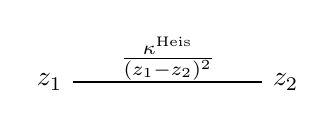
\begin{tikzpicture}
\node at (0,0) {$z_1$};
\node at (3,0) {$z_2$};
\draw[thick] (0.3,0) -- (2.7,0);
\node at (1.5, 0.3) {$\frac{\kappa^{\mathrm{Heis}}}{(z_1-z_2)^2}$};
\end{tikzpicture}
\end{center}

The genus-$0$ bar complex is computed on
$\overline{C}_n(\mathbb{P}^1)$ by logarithmic forms with coefficients
in $a(z_1)\otimes\cdots\otimes a(z_n)$; its differential is the
tree-level chiral factorization residue.  The bar differential uses
the logarithmic collision form
$\eta_{12}=d\log(z_1-z_2)$, the conformally invariant simple-pole
form along the diagonal.  It is
not multiplied with the Wick kernel to form a new meromorphic
propagator.  The residue operation is the chiral product:
\begin{equation}\label{eq:heisenberg-bar-residue-vol2}
d^{(0)}_{\mathrm{res}}[a\otimes a\otimes\eta_{12}]
= a_{(1)}a
= \kappa^{\mathrm{Heis}}\mathbf{1},
\end{equation}
because $a_{(0)}a=0$ and the double-pole coefficient is
$a_{(1)}a=\kappa^{\mathrm{Heis}}\mathbf{1}$ in the
Beilinson--Drinfeld chiral product convention~\cite[\S3.4]{BD04}.
Thus
$\operatorname{Res}_{D_{12}}$ denotes the chiral residue map, not the
ordinary meromorphic residue of
$\eta_{12}\cdot\kappa^{\mathrm{Heis}}(z_1-z_2)^{-2}$.  The Wick kernel
$G(z,w)$ remains the Gaussian contraction kernel in the BV model.

\section{The free boson at genus~\texorpdfstring{$1$}{1}}

On the elliptic curve
$E_\tau=\mathbb{C}/(\mathbb{Z}+\tau\mathbb{Z})$, the Gaussian
self-contraction gives
\begin{equation}\label{eq:heisenberg-tadpole-vol2}
A_{\mathrm{tad}}^{(E_\tau)}
= \kappa^{\mathrm{Heis}}\,G_2(\tau),\qquad
G_2(\tau):=\sideset{}{'}\sum_{(n,m)\in\mathbb{Z}^2}
\frac{1}{(n+m\tau)^2}
= \frac{\pi^2}{3}E_2(\tau).
\end{equation}
The normalized Eisenstein series satisfies
\[
E_2(-1/\tau)=\tau^2E_2(\tau)+\frac{6\tau}{\pi i},
\]
so the genus-$1$ scalar anomaly is proportional to
$\kappa^{\mathrm{Heis}}$.

\begin{center}
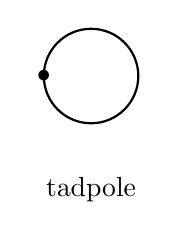
\begin{tikzpicture}[scale=1.2]
\node at (0,0) {$\bullet$};
\draw[thick] (0,0) arc (180:540:0.5);
\node at (0.5, -1.2) {tadpole};
\end{tikzpicture}
\end{center}

In the modular bar complex this trace is not a new
$d^{(0)}$-differential.  The Heisenberg cubic vertex vanishes, so the
stable-graph recursion has no cubic interaction term; the genus-$1$
scalar comes from the binary double-pole class transported through
the Hodge line:
\[
\operatorname{obs}_1(\mathcal{H}_{\kappa^{\mathrm{Heis}}})
= \kappa^{\mathrm{Heis}}\lambda_1,\qquad
F_1(\mathcal{H}_{\kappa^{\mathrm{Heis}}})
= \kappa^{\mathrm{Heis}}
\int_{\overline{\mathcal{M}}_{1,1}}\lambda_1
= \frac{\kappa^{\mathrm{Heis}}}{24}.
\]

\subsection{Loop-genus correspondence}

\begin{theorem}[Loop-genus correspondence {\cite{costello-renormalization}}]
\label{thm:loop-genus-correspondence}
A connected ribbon Feynman graph $\Gamma$ with $V$ vertices, $E$ edges,
and $F$ faces has loop number $L=E-V+1$.  The genus of the ribbon
surface satisfies
\[
\chi=V-E+F=2-2g,\qquad
g=\frac{L+1-F}{2}\leq \frac{L}{2},
\]
with equality when $F=1$.
\end{theorem}

The genus in $\bar{B}^{(g)}$ is the stable-curve genus.  In a ribbon
model it is bounded by graph loop number as above, but the
Heisenberg scalar obstruction is linear in the level:
\[
\operatorname{obs}_g(\mathcal{H}_{\kappa^{\mathrm{Heis}}})
= \kappa^{\mathrm{Heis}}\lambda_g,\qquad
F_g(\mathcal{H}_{\kappa^{\mathrm{Heis}}})
= \kappa^{\mathrm{Heis}}\lambda_g^{\mathrm{FP}}
\]
on the uniform-weight scalar lane
(Theorem~\ref{V1-thm:genus-universality} and
Theorem~\ref{thm:heisenberg-bv-bar-all-genera}).  The bar genus
filtration is not weighted by
$(\kappa^{\mathrm{Heis}})^g$.

\section{One-loop partition function}

The Gaussian path integral on $E_\tau$ gives
\[
Z_{E_\tau}=(\operatorname{Im}\tau)^{-1/2}|\eta(\tau)|^{-2},
\]
which is modular invariant as a density on $\mathcal{M}_{1,0}$.  The
bar complex does not identify this analytic function with a homology
group.  Its zero-mode-reduced vacuum line is
\[
H^0\bigl(\bar{B}^{(1)}
(\mathcal{H}_{\kappa^{\mathrm{Heis}}})\bigr)=\mathbb{C},
\]
and its scalar anomaly is
\[
F_1(\cA)=\kappa(\cA)\deg(\lambda_1)=\frac{\kappa(\cA)}{24}
\]
(Theorems~\ref{V1-thm:genus-universality}
and~\ref{V1-thm:explicit-theta}).

\section{The Gaussian comparison and the interacting obstruction}

\begin{proposition}[Heisenberg Gaussian BV/bar package]
\label{prop:heisenberg-gaussian-bv-bar-package}
Let $\mathcal{H}_{\kappa^{\mathrm{Heis}}}$ be the Heisenberg vertex
algebra at nonzero level on a compact Riemann surface~$\Sigma_g$.
Let
\[
C^\bullet_{\mathrm{BV,red}}
(\Sigma_g;\mathcal{H}_{\kappa^{\mathrm{Heis}}})
\]
be the zero-mode-reduced Gaussian BV complex, and let
$\bar{B}^{(g)}_{\mathrm{geom}}
(\mathcal{H}_{\kappa^{\mathrm{Heis}}})$ be the geometric bar complex
with logarithmic collision forms and chiral residue differential.
Then the comparison data are:
\begin{enumerate}[label=\textup{(\roman*)}]
\item the genus-$0$ chain-level contraction class is
 \eqref{eq:heisenberg-bar-residue-vol2};
\item under holonomicity and excision, the geometric bar complex
 computes factorization homology,
 \[
 H_*\bigl(\bar{B}^{(g)}_{\mathrm{geom}}
 (\mathcal{H}_{\kappa^{\mathrm{Heis}}})\bigr)
 \cong
 \int_{\Sigma_g}\mathcal{H}_{\kappa^{\mathrm{Heis}}},
 \]
 by Ayala--Francis excision for factorization homology
 \cite[Theorem~5.1]{AF15} together with the
 Beilinson--Drinfeld chiral/factorization correspondence
 \cite[\S3.4]{BD04};
\item the reduced free-field bar complex is quasi-isomorphic to the
 chain-level Gaussian BV complex for free fields
 \cite[Ch.~4, Thm.~4.4.1]{CG17}, and the scalar
 all-genera free energy satisfies
 \[
 F_g^{\mathrm{BV}}(\mathcal{H}_{\kappa^{\mathrm{Heis}}})
 =
 F_g^{\mathrm{bar}}(\mathcal{H}_{\kappa^{\mathrm{Heis}}})
 =
 \kappa^{\mathrm{Heis}}\lambda_g^{\mathrm{FP}}
 \]
 for $g\geq 1$
 (Theorem~\ref{thm:heisenberg-bv-bar-all-genera}).
\end{enumerate}
For $g\geq 1$ the bar cohomology groups are those of
Theorem~\ref{V1-thm:heisenberg-higher-genus}.
\end{proposition}

\begin{proof}
Part~\textup{(i)} is the direct Heisenberg OPE computation: the
bar differential applies the chiral product $a_{(1)}a$, not an
ordinary residue of a product of kernels.  Part~\textup{(ii)} is the
Ayala--Francis factorization-homology comparison for the geometric
bar model under the stated finiteness and excision hypotheses.  The
free-field BV comparison in part~\textup{(iii)} is Gaussian: all
connected correlators are obtained by Wick contractions, and the
bar side has only the binary residue \eqref{eq:heisenberg-bar-residue-vol2}.
The scalar equality is exactly Theorem~\ref{thm:heisenberg-bv-bar-all-genera}.
\end{proof}

\begin{theorem}[Interacting BV/bar obstruction]
\label{thm:interacting-bv-bar-obstruction}
Let $\cA$ be a chirally Koszul chiral algebra, and let
$g\geq 1$.  Let
\[
f_g\colon C^\bullet_{\mathrm{BV}}(\cA,\Sigma_g)\longrightarrow
B^{(g)}(\cA)
\]
be the filtered curved comparison morphism of
Theorem~\ref{thm:bv-bar-coderived}.  Choose the Hodge decomposition of
the BV propagator
\[
P_{\mathrm{BV}}
= d\log E + [d_{\mathrm{fib}},h] + P_{\mathrm{harm}},
\]
where $E$ is the prime form, $h$ is the fiberwise contracting
homotopy, and $P_{\mathrm{harm}}$ is the harmonic projection.  The
commutator term is a chain homotopy.  The obstruction to upgrading
the coderived comparison to a filtered chain-level comparison is
represented in filtration~$r$ by
\[
\operatorname{Ob}_r(\cA,g)
= [\delta_r^{\mathrm{harm}}]
\in
H^2\!\left(
\gr^r\Defcyc^{\mathrm{mod}}(\cA),
d_\Theta
\right),
\qquad
d_\Theta=d_{\Defcyc}+[\Theta_{\cA,0},{-}].
\]
A chain-level comparison requires, for every stable-graph component
of $\delta_r^{\mathrm{harm}}$, a primitive
$H_{\Gamma,r}$ satisfying
\[
d_\Theta H_{\Gamma,r}
=\delta_{\Gamma,r}^{\mathrm{harm}},
\]
with these primitives compatible with edge contraction, separating
gluing, and the codimension-$2$ stable-graph cancellations of
Construction~\ref{constr:feynman-stable-graph}.

The consequences are:
\begin{enumerate}[label=\textup{(\roman*)}]
\item for classes $\mathsf{G}$ and $\mathsf{L}$,
 $\delta_r^{\mathrm{harm}}=0$ for all $r$, so $f_g$ is a weak
 equivalence of filtered curved models;
\item for class $\mathsf{C}$, the same conclusion holds precisely
 under harmonic decoupling;
\item for class $\mathsf{M}$,
 \[
 \delta_r^{\mathrm{harm}}
 =
 c_r(\cA)\,m_0^{\lfloor r/2\rfloor-1}
 \qquad (r\geq 4),
 \]
 and the cone of $f_g$ is coacyclic.  Hence the comparison is an
 isomorphism in $D^{\mathrm{co}}$, while a direct-sum chain-level
 comparison still requires the primitives $H_{\Gamma,r}$ above.
\end{enumerate}
\end{theorem}

\begin{proof}
Theorem~\ref{thm:bv-bar-coderived} gives the comparison morphism
$f_g$ and the Hodge decomposition
$P_{\mathrm{BV}}=d\log E+[d_{\mathrm{fib}},h]+P_{\mathrm{harm}}$.
The commutator term changes the comparison by the displayed
homotopy.  The remaining failure to intertwine the curved
differentials is exactly the harmonic discrepancy
$\delta^{\mathrm{harm}}=\sum_r\delta_r^{\mathrm{harm}}$.  Passing to
the associated graded of the filtration puts each component in the
degree-$2$ cohomology group displayed above; a correction at stage
$r$ is precisely a primitive $H_{\Gamma,r}$ for that component,
compatible with the stable-graph differential.  The three
class-by-class clauses are the corresponding clauses of
Theorem~\ref{thm:bv-bar-coderived}.
\end{proof}

\begin{problem}[Interacting path-integral comparison datum]
\label{prob:interacting-path-integral-comparison-datum}
For an interacting chiral algebra $\cA$, construct a renormalized
BV factorization model $\mathcal{F}_{\cA,g}$, a genus-completed
filtered $L_\infty$ morphism
\[
\Phi_g^{\mathrm{BV/bar}}\colon
\mathcal{F}_{\cA,g}\longrightarrow \bar{B}^{\mathrm{ch},g}(\cA),
\]
and stable-graph homotopies $H_{\Gamma,r}$ satisfying the equations
of Theorem~\ref{thm:interacting-bv-bar-obstruction}.  The morphism
must restrict at $g=0$ on the anomaly-free Kac--Moody locus to the
quasi-isomorphism of Theorem~\ref{thm:brst-bar-genus0}, and its
degree-$2$ scalar projection must recover
$\Theta_\cA^{\leq 2}=\kappa(\cA)\cdot\eta\otimes\Lambda$ as in
Theorem~\ref{V1-thm:explicit-theta}.  The datum is not a determinant
formula for the bar complex; it is a compatible system of
propagator replacement maps, graphwise homotopies, and obstruction
classes.
\end{problem}

\begin{remark}[Shadow depth in the Feynman picture]
\label{rem:feynman-depth-decomposition}
Theorem~\ref{thm:loop-genus-correspondence} supplies only a graph
bound.  The algebraic invariant in the shadow tower is
\[
r_{\max}(\cA)=\sup\{r\geq 2:\cA^{\mathrm{sh}}_{r,0}\neq 0\},
\]
not the loop order of a chosen perturbative model
(Theorem~\ref{thm:shadow-archetype-classification}).  A Feynman
drawing of $S_r(\cA)$ is a stable-graph contact term of arity~$r$,
not a connected $(r-1)$-loop amplitude.
\end{remark}

\begin{remark}[Scope of the bar-path-integral comparison]
\label{rem:bar-path-integral-scope}
The Heisenberg comparison in
Proposition~\ref{prop:heisenberg-gaussian-bv-bar-package} is the
Gaussian, zero-mode-reduced, chain-level comparison together with the
factorization-homology and scalar all-genera data stated there.  For
interacting chiral algebras $\cA$, the all-genera statement is the
coderived comparison of Theorem~\ref{thm:bv-bar-coderived};
the direct chain-level comparison is controlled by
Theorem~\ref{thm:interacting-bv-bar-obstruction} and
Problem~\ref{prob:interacting-path-integral-comparison-datum}.

All Arnold-relation and sign checks occur in the ordered $E_1$ lift
before averaging.  The symmetric modular class is obtained after
quotienting labelled configurations by the symmetric group; the
stable-graph automorphism denominators in
Construction~\ref{constr:feynman-stable-graph} belong to this averaged
surface.  The path-integral comparison is separate from the three
structural identifications in the spine of the monograph:
$\Omega^{\mathrm{ch}}\bar{B}^{\mathrm{ch}}(\cA)\simeq\cA$ is
bar-cobar inversion, $\mathbb{D}_{\Ran}\bar{B}_X(\cA_i)\simeq\cA^!$
is Verdier duality, and $Z^{\mathrm{der}}_{\mathrm{ch}}(\cA)$ is
governed by chiral Hochschild cochains
(Theorem~\ref{thm:three-hochschild-unification}).
\end{remark}
